\documentclass[12pt]{standalone}
\usepackage{tikz}
\usetikzlibrary{automata,positioning}

\begin{document}
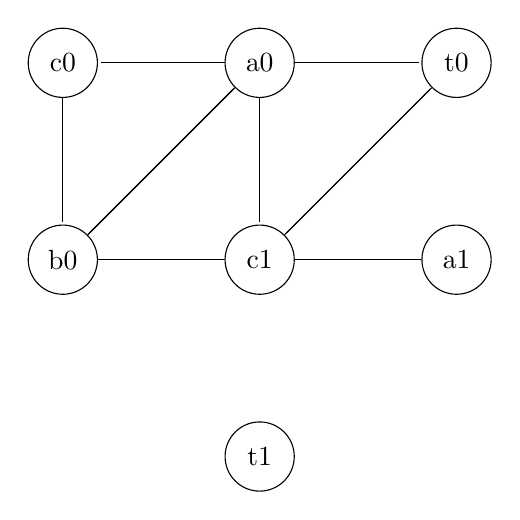
\begin{tikzpicture}[shorten >=1pt,node distance=2.5cm,on grid,auto] 

   \node[state] (c0)   {c0}; 
   \node[state] (a0) [right=of c0] {a0}; 
   \node[state] (t0) [right=of a0] {t0}; 
   \node[state] (c1) [below=of a0] {c1};
   \node[state] (b0) [below=of c0, left=of c1] {b0}; 
   \node[state] (a1) [below=of t0, right=of c1] {a1}; 
   \node[state] (t1) [below=of c1] {t1}; % t1 est présent mais sans lien

   % Liens pour a0 : t0 b0 c0 c1
   \path[-] (a0) edge (t0);
   \path[-] (a0) edge (b0);
   \path[-] (a0) edge (c0);
   \path[-] (a0) edge (c1);

   % Liens pour t0 : a0 c1
   \path[-] (t0) edge (c1);

   % Liens pour c0 : a0 b0
   \path[-] (c0) edge (b0);

   % Liens pour b0 : c0 a0 c1
   \path[-] (b0) edge (c1);
   \path[-] (b0) edge (a0);

   % Lien pour a1 : c1
   \path[-] (a1) edge (c1);

   % Lien pour c1 : a0 t0 a1 b0
   \path[-] (c1) edge (t0);
   \path[-] (c1) edge (a1);
   \path[-] (c1) edge (b0);

\end{tikzpicture}
\end{document}
